

\chapter{Implementation, Testing \& Result Analysis}\label{chap4}



\vspace*{40 ex}
%============================================================
\paragraph*{Outline:} This chapter presents the following:
\begin{enumerate}
\setlength{\itemsep}{-0.3em}
\item A brief of hardware implementation
\item A brief of software implementation
\item Testing of the project
\item Final result Analysis
\end{enumerate}
%============================================================

\newpage

\section{Hardware Implementation}

A hardware implementation means that the job is done using a physical device or electronic circuit as opposed to being done by a computer program. A hardware implementation often takes longer to create and that can make it more expensive. Hardware implementation is the building of the blocks of digital chip (either ASIC or FPGA) design and it relates them to the hardware description languages that are used in their creation

\subsection{Block Diagram}

\begin{figure}[!ht]
\centering
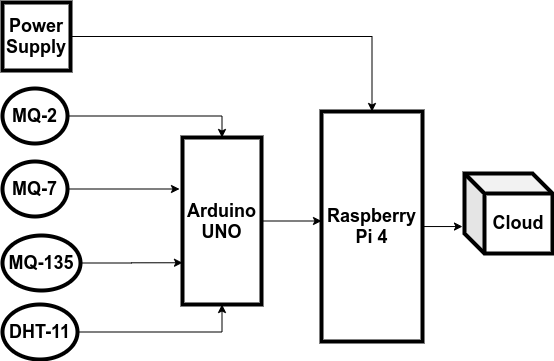
\includegraphics[width=\linewidth]{figures/arc-diagram.png}
\caption{\label{img41} An Architectural Diagram of the system.}
\end{figure}


\subsection{Flow Chart}

The flow of data should be cleared for every data processing unit and this study proposes a flow of data with simple and straight forward explanations which can see in figure~\ref{img42}. In this flow chart it's shown that every gas sensors and temperature have some threshold and if the value that are coming from sensors is less than given unit then it's counted as error and the value will be discarded.

\begin{figure}[!ht]
\centering
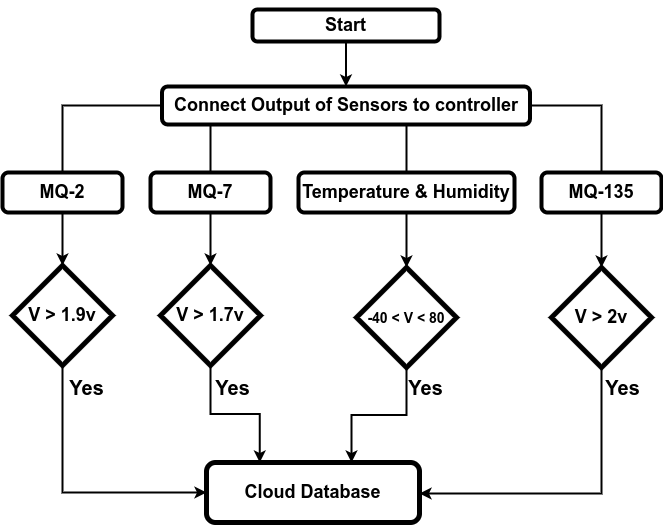
\includegraphics[width=\linewidth]{figures/flow-chart.png}
\caption{\label{img42} Flow of data from sensors to cloud database}
\end{figure}



\section{Software Implementation}

The software implementation stage involves the transformation of the software technical data package (TDP) into one or more fabricated, integrated, and tested software configuration items that are ready for software acceptance testing. The primary activities of software implementation include fabrication of software units to satisfy structural unit specifications, Assembly, integration, and testing of software components into a software configuration item.


\subsection{Hardware Data to cloud}

\subsubsection{Data Collection from MQ-2 sensor through Arduino Sketch}

\begin{lstlisting}[language=C, caption= Data calibration from MQ-2 Sensor]
const int inputPin = A0;
float R0;
int i = 1;
float LPGCurve[3] = {2.3,0.21,-0.47}; 
float COCurve[3] = {2.3,0.72,-0.34};
float SmokeCurve[3] = {2.3,0.53,-0.44}; 

void setup() {
  Serial.begin(9600);
  pinMode(inputPin, INPUT); 
  R0 = R0Calculate();
  delay(10000);
}

void loop() {
  float sensor_volt;
  float RS_gas; 
  float ratio; 

  float sensorValue = analogRead(inputPin); 
  
  sensor_volt = sensorValue*(5.0/1023.0);
  RS_gas = ((5.0*10.0)/sensor_volt)-10.0; 
  ratio = RS_gas/R0;  
  
  double  LPG = MQGetPercentage(ratio,LPGCurve);
  Serial.print(LPG);
  Serial.print(",");
  
  double  CO = MQGetPercentage(ratio,COCurve);
  Serial.print(CO);
  Serial.print(",");

  double  Smoke = MQGetPercentage(ratio,SmokeCurve);
  Serial.println(Smoke);
  delay(1000);
}

float R0Calculate(){
  float RS_air; 
  float R0;
  float sensorValue=0.0;
  float sensor_volt;
  
  for(int x = 0 ; x < 10000 ; x++) {
    sensorValue = sensorValue + analogRead(A0);
  }

  sensorValue = sensorValue/10000.0;
  sensor_volt = sensorValue*(5.0/1023.0); 
  RS_air = ((5.0*10.0)/sensor_volt)-10.0;
  R0 = RS_air/3.7;
  return R0;
}

double  MQGetPercentage(float rs_ro_ratio, float *pcurve) {
  return (pow(10,( ((log(rs_ro_ratio)-pcurve[1])/pcurve[2]) + pcurve[0])));
}

\end{lstlisting}


\subsubsection{Data calibration from Serial Port}
The most important part of calibration is watching the readings during the calibration process. It is easiest to calibrate the device in its default state (UART mode, with continuous readings enabled). Switching the device to I2C mode after calibration will not affect the stored calibration. If the device must be calibrated in I2C mode be sure to continuously request readings so you can see the output from the serial port, here we have initialized the baudrate 9600 that's best suited for Arduino UNO.

\begin{lstlisting}[language=Python, caption= Data calibration from Arduino Serial port]

import serial
from datetime import datetime
import firebase_admin
from firebase_admin import credentials
from firebase_admin import firestore

cred = credentials.Certificate("firebase-key.json")
firebase_admin.initialize_app(cred)
db = firestore.client()
col_ref = db.collection('coliberation')
ser = serial.Serial('/dev/ttyACM2',baudrate=9600,timeout=1)

while True:
    arduinoData = ser.readline().decode('ascii')
    sensorValue = arduinoData.split(',')

    if len(sensorValue)==3:
        LPG = float(sensorValue[0])
        _ = float(sensorValue[1])
        smoke = float(sensorValue[2])
        CO = float(sensorValue[3])
        airquality = float(sensorValue[4])
        CO2 = float(sensorValue[5])
        NH4 = float(sensorValue[6])
        temperature = float(sensorValue[7])
        humidity = float(sensorValue[8])
        data = {
            "time" : datetime.now(),
            "LPG" : LPG,
            "CO" : CO,
            "smoke" : smoke,
            "temperature" : temperature,
            "humidity" : humidity,
            "airquality" : airquality,
            "CO2" : CO2,
            "NH4" : NH4 
        }
        col_ref.add(data)
\end{lstlisting}

\subsection{ML Integration for Weather Forecast Prediction}

Weather forecasting is the application of science and technology to predict the conditions of the atmosphere for a given location and time. People have attempted to predict the weather informally for millennia and formally since the $19^{th}$ century. Weather forecasts are made by collecting quantitative data about the current state of the atmosphere at a given place and using meteorology to project how the atmosphere will change.

Once calculated by hand based mainly upon changes in barometric pressure, current weather conditions, and sky condition or cloud cover, weather forecasting now relies on computer-based models that take many atmospheric factors into account. Human input is still required to pick the best possible forecast model to base the forecast upon, which involves pattern recognition skills, teleconnections, knowledge of model performance, and knowledge of model biases. The inaccuracy of forecasting is due to the chaotic nature of the atmosphere, the massive computational power required to solve the equations that describe the atmosphere, the error involved in measuring the initial conditions, and an incomplete understanding of atmospheric processes. Hence, forecasts become less accurate as the difference between current time and the time for which the forecast is being made (the range of the forecast) increases. 

There is a vast variety of end uses to weather forecasts. Weather warnings are important forecasts because they are used to protect life and property. Forecasts based on temperature and precipitation are important to agriculture, and therefore to traders within commodity markets. Temperature forecasts are used by utility companies to estimate demand over coming days.

\subsubsection{Dataset and Data Preprocessing}

This dataset contains 6 different features such as air temperature, atmospheric pressure, humidity, Windspeed and WindDirection. These were collected every 1 hour, beginning on 29 May 2020 to ending on 12 June 2020. This section of the dataset was collected from meteoblue(https://www.meteoblue.com/en/weather) that consists of 328 time series data. 

It is important to scale features before training a neural network. Standardization is a common way of doing this scaling by subtracting the mean and dividing by the standard deviation of each feature. 

The data preprocessing is being done by standard method,
Suppose there are n number of data points present in dataset and their values are $X_1, X_2, X_3, X_4, X_5 ....., X_n$ and $X_{mean}$ is a mean of all data points and $X_{dev}$ is a standard deviation of all data points and their calculation is following 

\[ X_{mean} = \dfrac{X_1 + X_2 + X_3 + X_4 + X_5 + ....... + X_n }{n} \]
\[X_{dev}^{2} = \sqrt{ ( X_1 -X_{mean} + X_2 -X_{mean} + X_3 -X_{mean} + .... + X_n -X_{mean} )^2}\]
\[ X_i = \dfrac{X_i - X_{mean}}{X_{dev}} i = 1, 2, 3, ..., n\]

\subsubsection{Model}
This study use LSTM model which is a deep
learning model proposed by Schmidhuber (Hochreiter
and Schmidhuber, 1997). The model has been
successfully used in many research fields such as,
large scale image classification (Real et al., 2017),
video classification (Yoo, 2017), natural language
processing (Elkaref and Bohnet, 2017), anomaly
detection (Luo et al., 2017; Lee et al., 2018). LSTM
was used as a foundation for weather forecasting
model because of several reasons that are the
model ability to solve long lag relationship in time
series data (2) the model ability to address vanisihing
gradient problems that occur in the training deep
structure neural networks (Gers et al, 2000). 

LSTM is a recurrence Neural Network that first
introduced by (Hochreiter and Schmidhuber, 1997) as a
specific Recurrent Neural Network (RNN) architecture that was designed to model temporal sequences. Better
than the conventional RNN, LTSTM is able to sort error
backflow problem so that this algorithm only use the
error feedback that can make more accurate prediction
whereas all unsupported feedback are removed. This
algorithm has sorting capability due to LSTM contains
special units called memory blocks in the recurrent
hidden layer. The LSTM overcome the weakness in
conventional RNN that show backpropagation algorithm
in RNNs cause error signals that flows backward in time
tend to explode or diminish; therefore, the temporal
evolution of the backpropagated error exponentially
depends on the size of the weight. In other words, the
strength of LSTM is special units called memory blocks
in the recurrent hidden layer. 

As we know that any Machine Learning(ML) or Deep Learning(DL) can only predict one feature although we can provide multiple features as input and based on those input features and also depends upon past history any model predict future data but the weather forecast needs multiple features like temperature, pressure, humidity, wind-speed and many more that is why this this project really needs more than one model to predict multiple features.

This entire modelling part is divided into three sub sections

\begin{itemize}
\item section 1: The prediction of temperature with univariate feature and timestamp as an input feature for prediction.

\item section 2: The prediction of humidity with univariate feature and timestamp as an input feature for prediction.

\item section 3: The prediction of pressure with univariate feature and timestamp as an input feature for prediction.
\end{itemize}

\subsubsection{Flow Chart}
The flow of data should be cleared for every data processing unit and this study proposes a flow of data with simple and straight forward explanations which can see figure~\ref{img43}.

\begin{figure}[!ht]
\centering
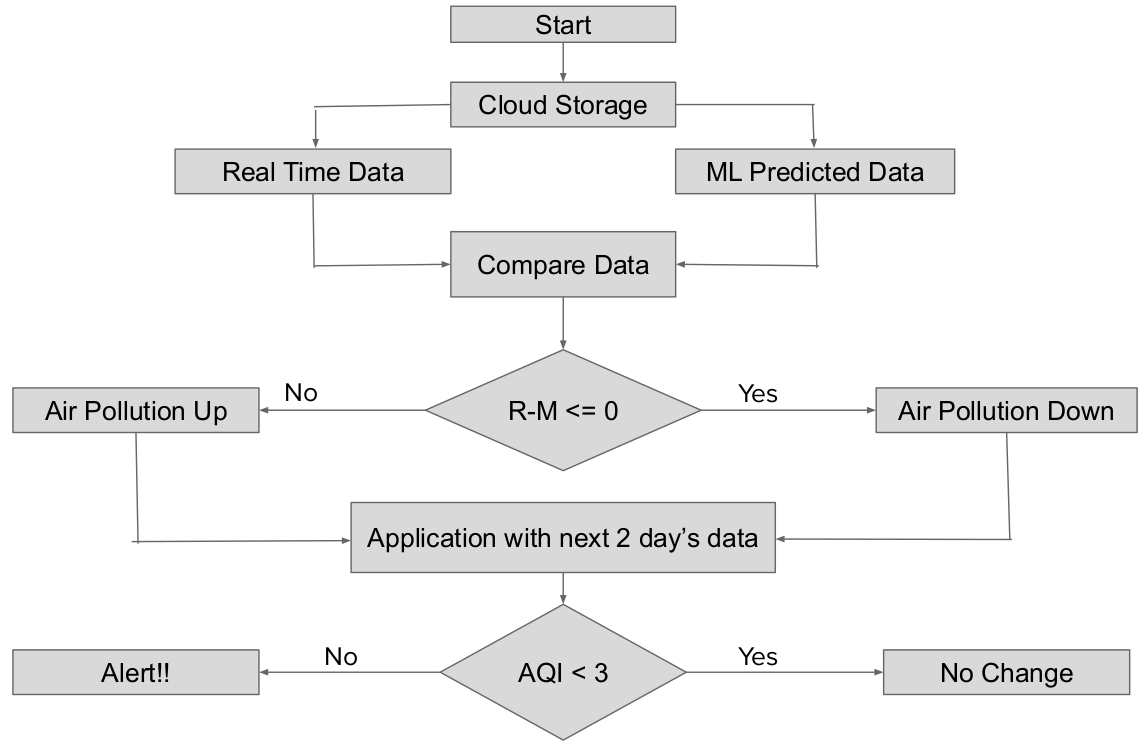
\includegraphics[width=\linewidth]{figures/ml-flow-chart.png}
\caption{\label{img43} flow of real time data with predicted data}
\end{figure}

\subsubsection{Logic Implementation}

\begin{figure}[!ht]
\centering
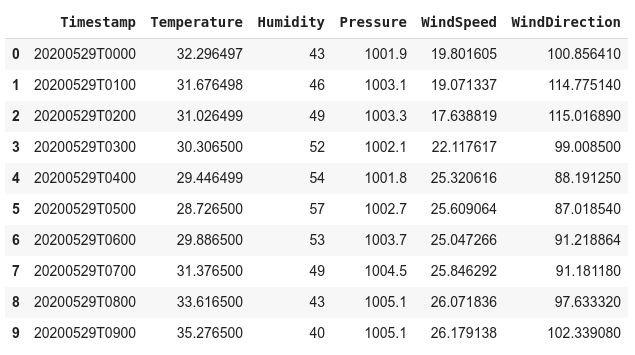
\includegraphics[width=\linewidth]{figures/sample-data.png}
\caption{\label{img44} sample of every an hour data}
\end{figure}

As you can see in figure~\ref{img44}, an observation is recorded every 1 hours. This means that, for a single hour, you will have only 1 observations. Similarly, a single day will contain 24 (1x24) observations.

Given a specific time, let's say you want to predict the temperature 6 hours in the future. In order to make this prediction, you choose to use 5 days of observations. Thus, you would create a window containing the last 120(5x24) observations to train the model. Many such configurations are possible, making this dataset a good one to experiment with.

The function below returns the above described windows of time for the model to train on. The parameter history\_size is the size of the past window of information. The target\_size is how far in the future does the model need to learn to predict. The target\_size is the label that needs to be predicted.

\begin{lstlisting}[language=Python, caption= A function to return windows of time followed by history\_size ]
def univariate_data(dataset, start_index, end_index, history_size, target_size):
  data = []
  labels = []
  start_index = start_index + history_size
  if end_index is None:
    end_index = len(dataset) - target_size
  for i in range(start_index, end_index):
    indices = range(i-history_size, i)
    # Reshape data from (history_size,) to (history_size, 1)
    data.append(np.reshape(dataset[indices], (history_size, 1)))
    labels.append(dataset[i+target_size])
  return np.array(data), np.array(labels)
\end{lstlisting}

It is important to scale features before training a neural network. Standardization is a common way of doing this scaling by subtracting the mean and dividing by the standard deviation of each feature.You could also use a tf.keras.utils.normalize method that rescales the values into a range of [0,1]. Note: The mean and standard deviation should only be computed using the training data.

\begin{lstlisting}[language=Python, caption= Scaling the feature by standard method]
uni_train_mean = uni_data[:TRAIN_SPLIT].mean()
uni_train_std = uni_data[:TRAIN_SPLIT].std()
uni_data = (uni_data-uni_train_mean)/uni_train_std
\end{lstlisting}

Let's now create the data for the univariate model. For our first model, the model will be given the last 20 recorded temperature observations, and needs to learn to predict the temperature at the next time step.

\begin{lstlisting}[language=Python, caption= Splitting data into training-set and validation-set]
univariate_past_history = 20
univariate_future_target = 0

x_train_uni, y_train_uni = univariate_data(uni_data, 0, TRAIN_SPLIT,
                                           univariate_past_history,
                                           univariate_future_target)
x_val_uni, y_val_uni = univariate_data(uni_data, TRAIN_SPLIT, None,
                                       univariate_past_history,
                                       univariate_future_target)
\end{lstlisting}

due to less availability of data our long short term memory(LSTM) model is simple and with the less number of happen layers and dense layers because adding more layers may lead to overfit or underfit this is something which we don't want. There summary of our model can see in figure~\ref{img45}

\begin{lstlisting}[language=Python, caption= Creating a LSTM model with their summary]
simple_lstm_model = tf.keras.models.Sequential([
    tf.keras.layers.LSTM(8, input_shape=x_train_uni.shape[-2:]),
    tf.keras.layers.Dense(1)
])

simple_lstm_model.compile(optimizer='adam', loss='mae')
simple_lstm_model.summary()

\end{lstlisting}

\begin{figure}[!ht]
\centering
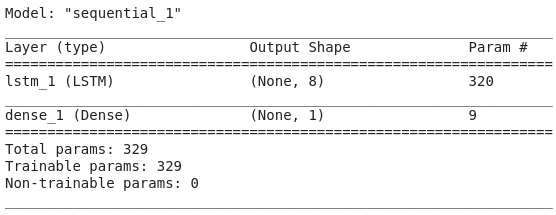
\includegraphics[width=\linewidth]{figures/model-summary.png}
\caption{\label{img45} Summary of simple long short term memory model}
\end{figure}

\subsection{Flutter Application}
Flutter is an open-source UI software development kit created by Google. It is used to develop applications for Android, iOS, Windows, Mac, Linux, Google Fuchsia and the web from a single codebase.

The first version of Flutter was known as codename "Sky" and ran on the Android operating system. It was unveiled at the 2015 Dart developer summit, with the stated intent of being able to render consistently at 120 frames per second.

Flutter apps are written in the Dart language and make use of many of the language's more advanced features.Flutter runs in the Dart virtual machine which features a just-in-time execution engine. While writing and debugging an app, Flutter uses Just In Time compilation, allowing for "hot reload", with which modifications to source files can be injected into a running application. Flutter extends this with support for stateful hot reload, where in most cases changes to source code can be reflected immediately in the running app without requiring a restart or any loss of state.Release versions of Flutter apps are compiled with ahead-of-time (AOT) compilation on both Android and iOS, making Flutter's high performance on mobile devices possible.

\subsubsection{Fetching data from cloud}

StreamBuilder is a Widget that can convert a stream of user defined objects, to widgets. This takes two arguments stream and builder, that can convert the elements of the stream to widgets
Suppose, you have a Stream, that updates if there is any UI update (may be from user interaction, or may be resulted from network updates). If your “main” widget, includes a StreamBuilder, which listens to the stream, it can act as the element in charge of translating your states to views.

\begin{lstlisting}[language=java, caption = Getting data from cloud database to flutter UI]
StreamBuilder<QuerySnapshot>(
        stream: _database.snapshots(),
        builder: (BuildContext context, AsyncSnapshot<QuerySnapshot> snapshot) {
          if (snapshot.hasError)
            return new Text('Error: ${snapshot.error}');
          switch (snapshot.connectionState) {
            case ConnectionState.waiting: return new Text('Loading...');
            default:
              return ListView.builder(
                  shrinkWrap: true,
                  itemCount: snapshot.data.documents.length,
                  itemBuilder: (BuildContext context, int index) {
                    double temperature = snapshot.data.documents[index]['temperature'];
                    double humidity = snapshot.data.documents[index]['humidity'];
                    dynamic time = snapshot.data.documents[index]['time'].toDate();
                    return Card(
                        color: Colors.deepOrange[400],
                        elevation: 10,
                        shape: RoundedRectangleBorder(
                          borderRadius: BorderRadius.circular(15.0),
                        ),
                        child: new Row(
                          mainAxisAlignment: MainAxisAlignment.spaceEvenly,
                          mainAxisSize: MainAxisSize.max,
                          children: <Widget>[
                            layout("Temperature",temperature, "Time", time, "Humidity", humidity),
                          ],
                        )
                    );
                  });
          }
        },
      ),

\end{lstlisting}

\subsubsection{Fetching data from ML API}
Long-running tasks are common in mobile apps. The way this is handled in Flutter / Dart is by using a Future. A Future allows you to run work asynchronously to free up any other threads that should not be blocked. Like the UI thread.

A future is defined exactly like a function in dart, but instead of void you use Future. If you want to return a value from the Future then you pass it a type.

\begin{lstlisting}[language=java, caption = Getting data from ML API to flutter UI]
Future<dynamic> getPrediction(year,month,day,hour,minute,humidity) async{
    final url = '$baseUrl/date/?name=$year,$month,$day,$hour,$minute,$humidity';
    print('fetching $url');
    final res = await httpClient.get(url);
    if (res.statusCode != 200) {
      throw HTTPException(res.statusCode, "unable to fetch weather data");
    }
    final predictionData = json.decode(res.body);
    return predictionData;
  }
\end{lstlisting}

\subsubsection{Fetching data from Weather API}

Future operations are the operations which take time to perform and return the result later. To handle this problem, we use Asynchronous functions. Asynchronous operations let your program continue other operations while the current operation is being performed. Dart uses Future objects (futures) to represent the results of asynchronous operations. To handle these operations, we can use Async/await, but it is not possible to integrate async and await on widgets. So it is quite tricky to handle futures in widgets. To solve this problem flutter provided a widget called Future Builder.

\begin{lstlisting}[language=java, caption = Getting data from Weather API to flutter UI]
FutureBuilder(
        future: getData(DateTime.now(), humidity),
        builder: (context, snapshot){
              dynamic keys = snapshot.data.keys.toList();
              DateTime time = new DateTime.now();
              return ListView.builder(
                itemCount: snapshot.data.length,
                itemBuilder: (BuildContext context, int index) {
                  final temp = snapshot.data[keys[index]].round();
                  var newtime = time.add(new Duration(seconds: 60*index));
                  var now = timePormat(newtime.year, newtime.month, newtime.day, newtime.hour,newtime.minute);
                  return Card(
                      color: Colors.deepOrange[400],
                      elevation: 10,
                      shape: RoundedRectangleBorder(
                        borderRadius: BorderRadius.circular(15.0),
                      ),
                      child: Text('$temp $now'),
                      )
                  );
                },
              );
          }
        }
    );
\end{lstlisting}
\section{Testing \& Result Analysis}

From a proper analysis of positive points and constraints on the component, it can be safely concluded that the product is a highly efficient GUI based component and with accurate weather forecasting system. This system is working properly and meeting to most of the user requirements. This component can be easily plugged in many other systems.

The aim of the proposed system testing process was to determine all defects in the project .The program was subjected to a set of test inputs and various observations were made and based on these observations it will be decided whether the program behaves as expected or not.

Testing and result analysis of this proposed is done in following three parts.
\begin{itemize}
\item Gas and Temperature sensors testing
\item Forecasting Models testing
\item Flutter application testing
\end{itemize}

\subsection{Gas and Temperature Sensors}
Data calibration of this proposed system is done using gas and temperature sensors such as MQ-2 gas sensor, MQ-7 carbon monoxide sensor, MQ-135 air quality sensor and DHT-11 temperature and humidity sensor and the working of these sensors with their datasheet is already explained in section 3.2, there are following parameters are tested in above mention sensors.
\begin{itemize}
\item Temperature
\item Humidity
\item Air Quality
\item Carbon Monoxide Gas
\item Carbon Dioxide Gas
\item Ammonium Gas
\item LPG Gas
\item Smoke
\end{itemize}


\subsection{Temperature}
Temperature is a physical property of matter that quantitatively expresses hot and cold. It is the manifestation of thermal energy, present in all matter, which is the source of the occurrence of heat, a flow of energy, when a body is in contact with another that is colder.
DHT-11(temperature and humidity) sensor is used to calibrate temperature.
\begin{figure}[!ht]
\centering
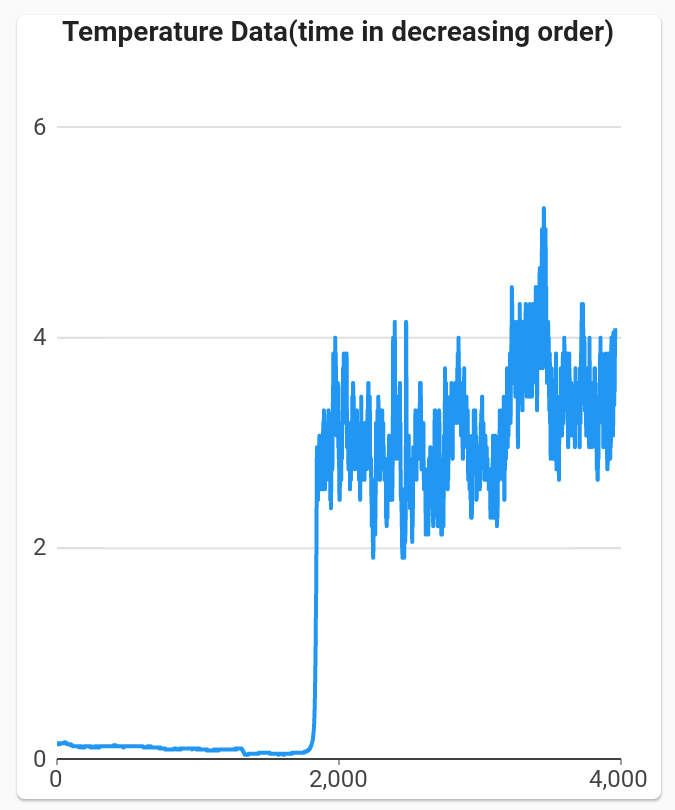
\includegraphics[width=\linewidth,height=8cm]{figures/temp.png}
\caption{\label{img46} Temperature variation with respect to time}
\end{figure}

\subsection{Humidity}
Humidity is the concentration of water vapor present in the air. Water vapor, the gaseous state of water, is generally invisible to the human eye. Humidity indicates the likelihood for precipitation, dew, or fog to be present. The amount of water vapor needed to achieve saturation increases as the temperature increases. As the temperature of a parcel of air decreases it will eventually reach the saturation point without adding or losing water mass. The amount of water vapor contained within a parcel of air can vary significantly. DHT-11(temperature and humidity) sensor is used to calibrate humidity.

\begin{figure}[!ht]
\centering
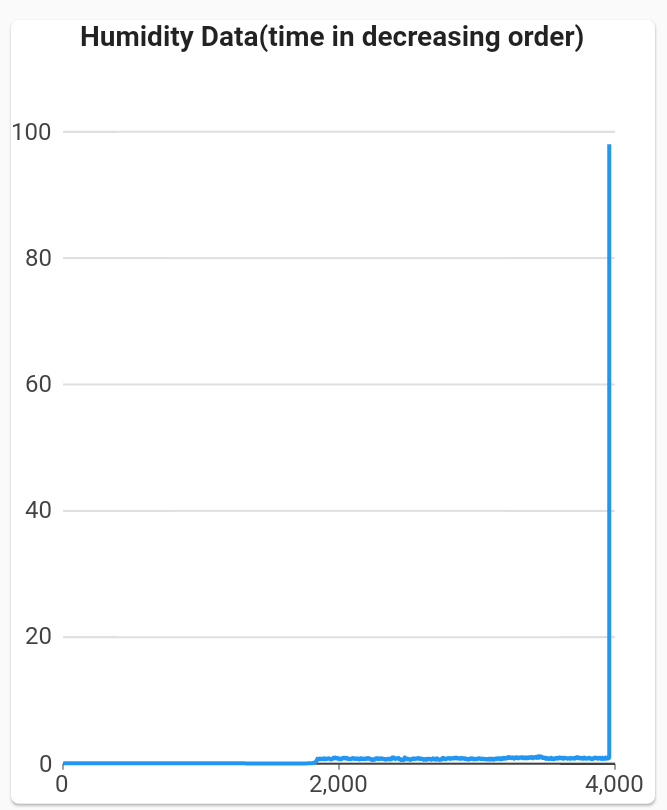
\includegraphics[width=\linewidth,height=8cm]{figures/humidity.png}
\caption{\label{img47} Humidity variation with respect to time}
\end{figure}

\subsection{Air Quality}
To measure air quality air quality index (AQI) unit is used.
An air quality index (AQI) is used by government agencies to communicate to the public how polluted the air currently is or how polluted it is forecast to become. Public health risks increase as the AQI rises. Different countries have their own air quality indices, corresponding to different national air quality standards. MQ-135 sensor is used to calibrate air quality.
\begin{figure}[!ht]
\centering
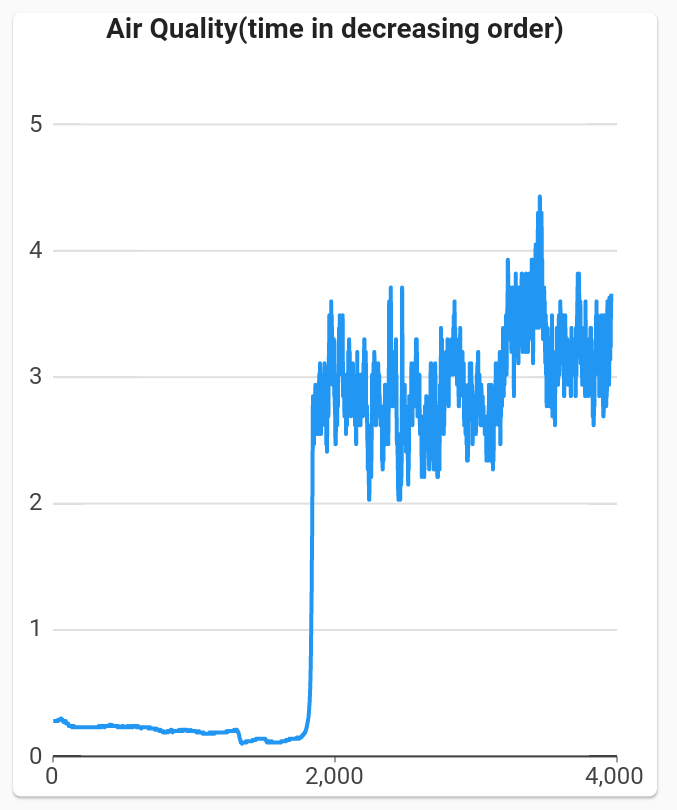
\includegraphics[width=\linewidth,height=8cm]{figures/airquality.png}
\caption{\label{img48} Air Quality variation with respect to time}
\end{figure}

\subsection{Carbon Monoxide Gas}
Carbon monoxide(CO) is a colorless, odorless, and tasteless flammable gas that is slightly less dense than air. It is toxic to animals that use hemoglobin as an oxygen carrier (both invertebrate and vertebrate) when encountered in concentrations above about 35 ppm, although it is also produced in normal animal metabolism in low quantities, and is thought to have some normal biological functions. In the atmosphere, it is spatially variable and short-lived, having a role in the formation of ground-level ozone. MQ-7 sensor is used to calibrate Carbon monoxide(CO).

\begin{figure}[!ht]
\centering
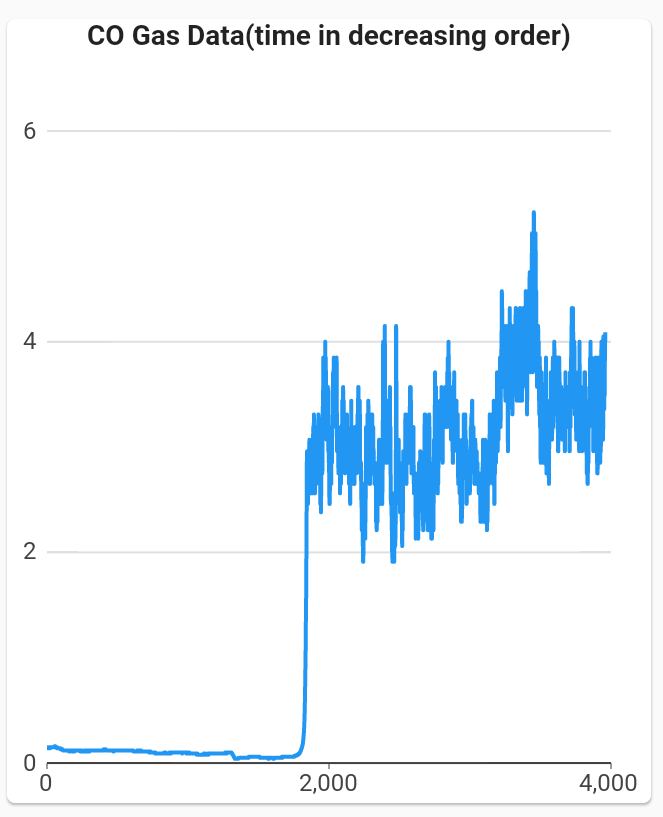
\includegraphics[width=\linewidth,height=8cm]{figures/CO.png}
\caption{\label{img49} Carbon Monoxide(CO) variation with respect to time}
\end{figure}

\subsection{Carbon Dioxide Gas}
Carbon dioxide is a colorless gas with a density about 60\% higher than that of dry air. Carbon dioxide consists of a carbon atom covalently double bonded to two oxygen atoms. It occurs naturally in Earth's atmosphere as a trace gas. The current concentration is about 0.04\% (412 ppm) by volume, having risen from pre-industrial levels of 280 ppm.[8] Natural sources include volcanoes, hot springs and geysers, and it is freed from carbonate rocks by dissolution in water and acids. Because carbon dioxide is soluble in water, it occurs naturally in groundwater, rivers and lakes, ice caps, glaciers and seawater.  MQ-2 sensor is used to calibrate Carbon Dioxide($CO_{2}$).
\begin{figure}[!ht]
\centering
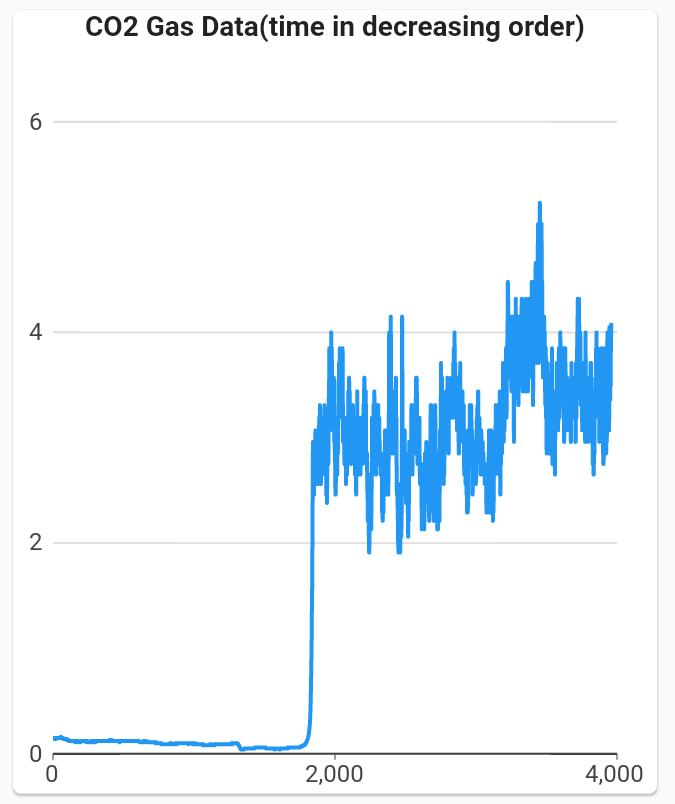
\includegraphics[width=\linewidth,height=8cm]{figures/CO2.png}
\caption{\label{img410} Carbon Dioxide($CO_{2}$) variation with respect to time}
\end{figure}

\subsection{Ammonium Gas}
Ammonia is a compound of nitrogen and hydrogen with the formula NH3. A stable binary hydride, and the simplest pnictogen hydride, ammonia is a colourless gas with a characteristic pungent smell. It is a common nitrogenous waste, particularly among aquatic organisms, and it contributes significantly to the nutritional needs of terrestrial organisms by serving as a precursor to food and fertilizers. Ammonia, either directly or indirectly, is also a building block for the synthesis of many pharmaceutical products and is used in many commercial cleaning products. It is mainly collected by downward displacement of both air and water.
\begin{figure}[!ht]
\centering
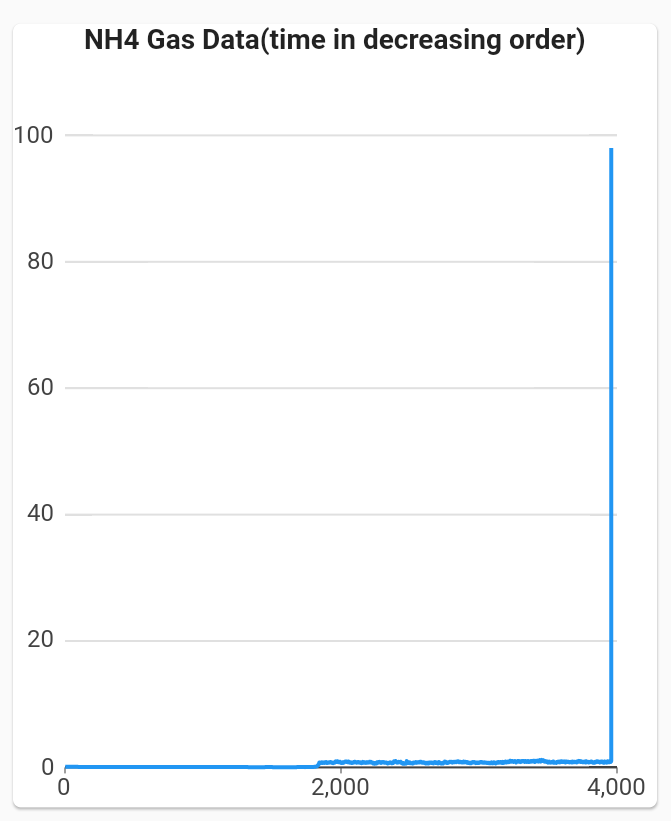
\includegraphics[width=\linewidth,height=8cm]{figures/NH4.png}
\caption{\label{img411} Ammonium($NH_{4}$) variation with respect to time}
\end{figure}

\subsection{LPG Gas}
Liquefied petroleum gas or liquid petroleum gas (LPG or LP gas), is a flammable mixture of hydrocarbon gases used as fuel in heating appliances, cooking equipment, and vehicles.

It is increasingly used as an aerosol propellant and a refrigerant, replacing chlorofluorocarbons in an effort to reduce damage to the ozone layer. When specifically used as a vehicle fuel it is often referred to as autogas.
\begin{figure}[!ht]
\centering
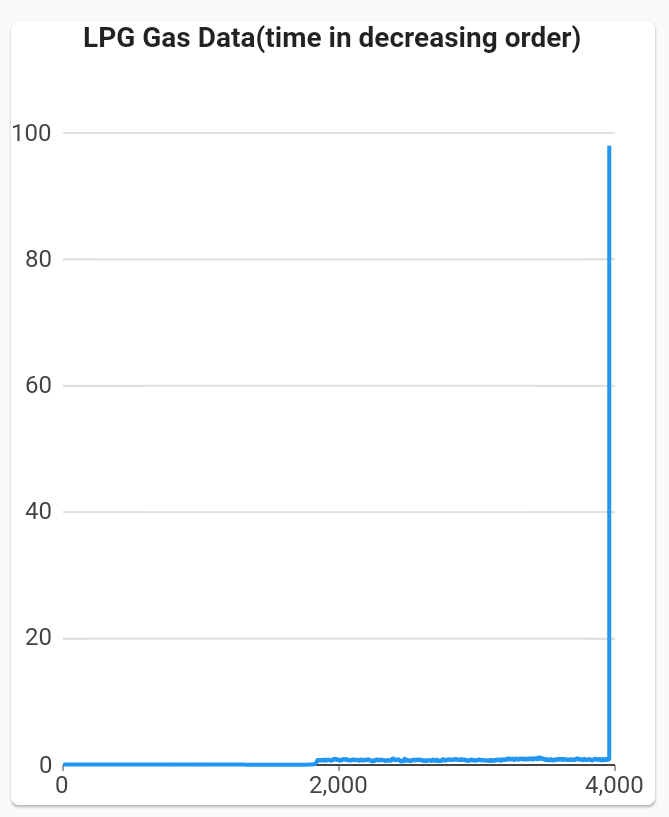
\includegraphics[width=\linewidth,height=8cm]{figures/LPG.png}
\caption{\label{img412} LPG variation with respect to time}
\end{figure}

\subsection{Smoke}
Smoke is a collection of airborne particulates and gases[1] emitted when a material undergoes combustion or pyrolysis, together with the quantity of air that is entrained or otherwise mixed into the mass. It is commonly an unwanted by-product of fires (including stoves, candles, internal combustion engines, oil lamps, and fireplaces), but may also be used for pest control (fumigation), communication (smoke signals), defensive and offensive capabilities in the military (smoke screen), cooking, or smoking (tobacco, cannabis, etc.). It is used in rituals where incense, sage, or resin is burned to produce a smell for spiritual or magical purposes. It can also be a flavoring agent and preservative for various foodstuffs.
\begin{figure}[!ht]
\centering
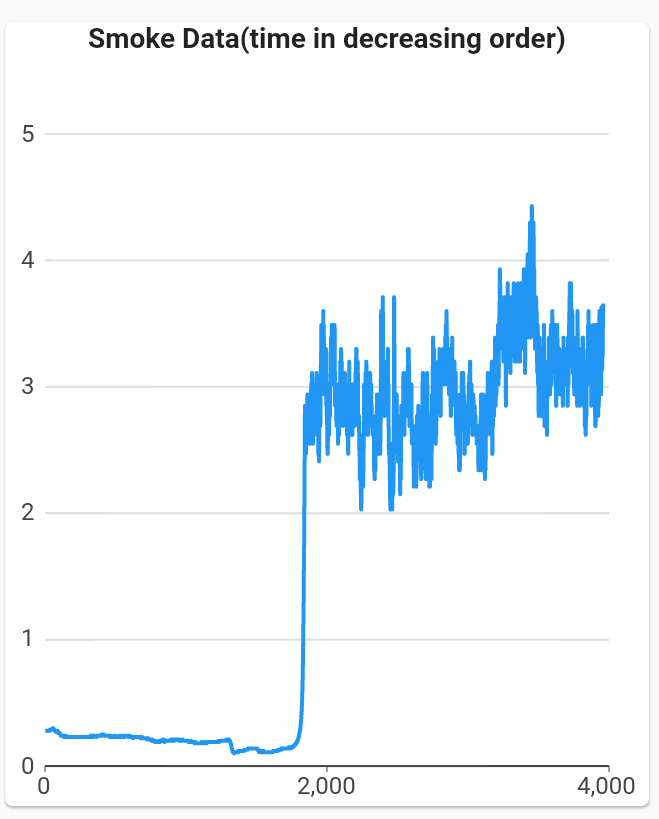
\includegraphics[width=\linewidth,height=8cm]{figures/smoke.png}
\caption{\label{img413} Smoke variation with respect to time}
\end{figure}


\subsection{Forecasting Models}
For the predicting weather forecast three different models are made. Model-1 is responsible for predicting temperature, model-2 is responsible for predicting humidity and model-3 is responsible for predicting pressure. The dataset and preprocesing part is explained in section 4.2.2.1, modelling part is explained in section 4.2.2.2 and the implementation of logic is explained in section 4.2.2.4, the table 4.1 summarizing models with their accuracy.

\begin{table}[!ht]
\centering
\begin{tabular}{ |p{2cm}|p{2cm}|p{2cm}|p{2cm}|p{2cm}| }
\hline
\multicolumn{5}{|c|}{Weather Forecasting Models} \\
\hline
Model&Feature&Training Data&Testing Data&Accuracy \\
\hline
Model-1&Temperature&80\%&20\%&73\%\\
Model-2 &Humidity&80\%&20\%&73\%\\
Model-3 &Pressure&80\%&20\%&73\%\\
\hline
\end{tabular}
\caption{\label{data}Weather models summary}
\end{table}

\subsection{Flutter Application}

The implementation of fetching data from cloud database, fetching data from Machine Learning, fetching data from Weather API, plotting the pollution status and comparison between ML model prediction and Weather API prediction are deeply explained in section 4.2.3, here it's tested that all the implemented features and component are working smoothly.

\subsection{Home Screen}
When the application get started figure~\ref{img414} screenshot page will be appearing, basically this has six ButtonTheme RadioButtons and every RadioButton is responsible of some activity like fetching data from cloud database, fetching data from weather API and many more activities.
\begin{figure}[!ht]
\centering
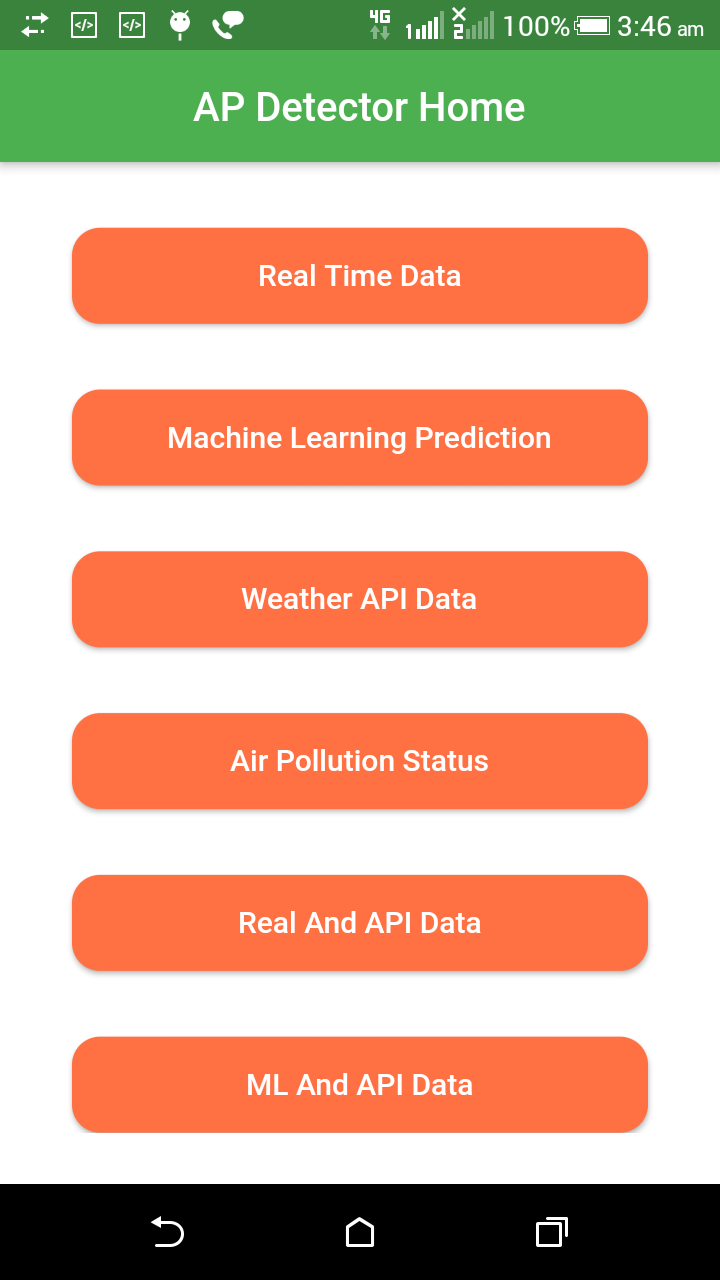
\includegraphics[height=10cm]{figures/home-screen.png}
\caption{\label{img414} Application home screen}
\end{figure}

\subsection{Real Time Data}
When will be pressing on first RadioButton then will go to figure~\ref{img415} screenshot page basically this page is showing real time data that are coming from all gas sensors and temperature sensor.

\begin{figure}[!ht]
\centering
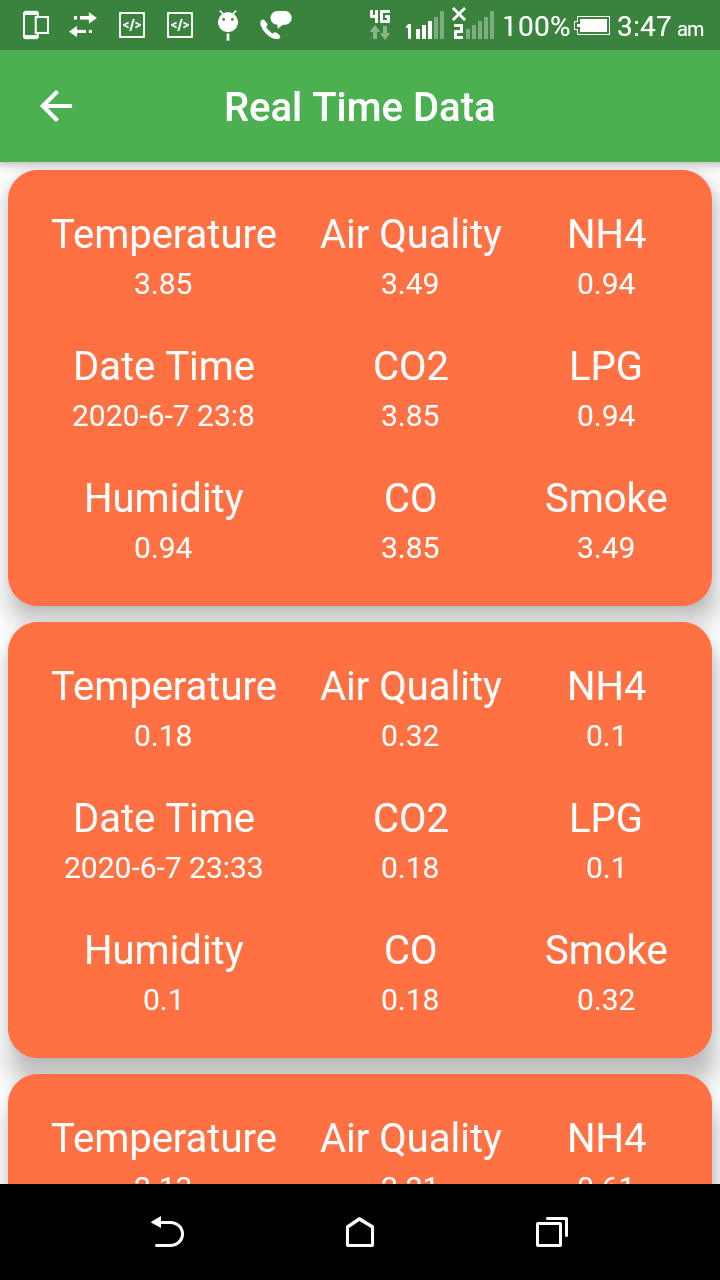
\includegraphics[height=10cm]{figures/real-data.png}
\caption{\label{img415} Real time data page}
\end{figure}

\subsection{ML Prediction Data}
When will be pressing on second RadioButton then will go to figure~\ref{img416} screenshot page basically this page is showing machine learning model prediction data that are coming from server. This page has next five day's weather forecast record which is after every 3 hours interval from current time. 

\begin{figure}[!ht]
\centering
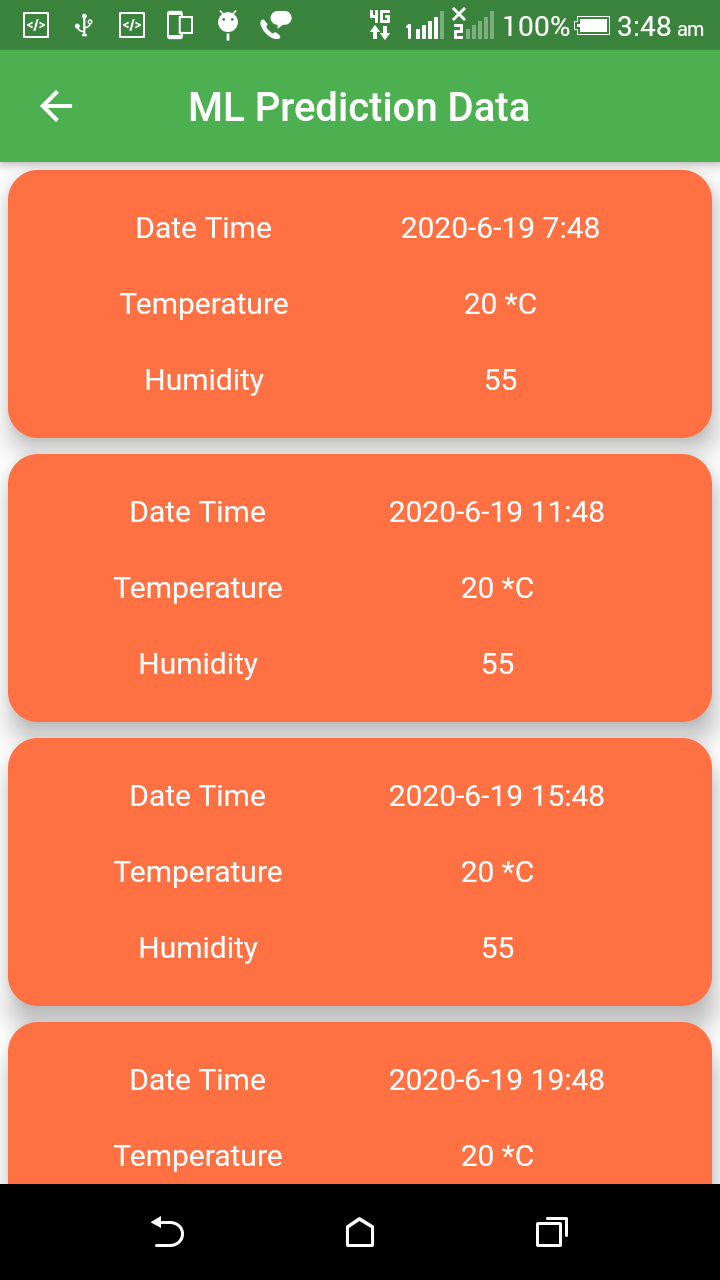
\includegraphics[height=10cm]{figures/ml-data.png}
\caption{\label{img416} ML prediction data page}
\end{figure}

\subsection{Weather API Data}
When will be pressing on third RadioButton then will go to figure~\ref{img417} screenshot page basically this page has two input field which are for latitude and longitude of current location, two RadioButtons first for current weather details and second for next five day's weather forecast and last one output field for showing details after pressing above two buttons.

\begin{figure}[!ht]
\centering
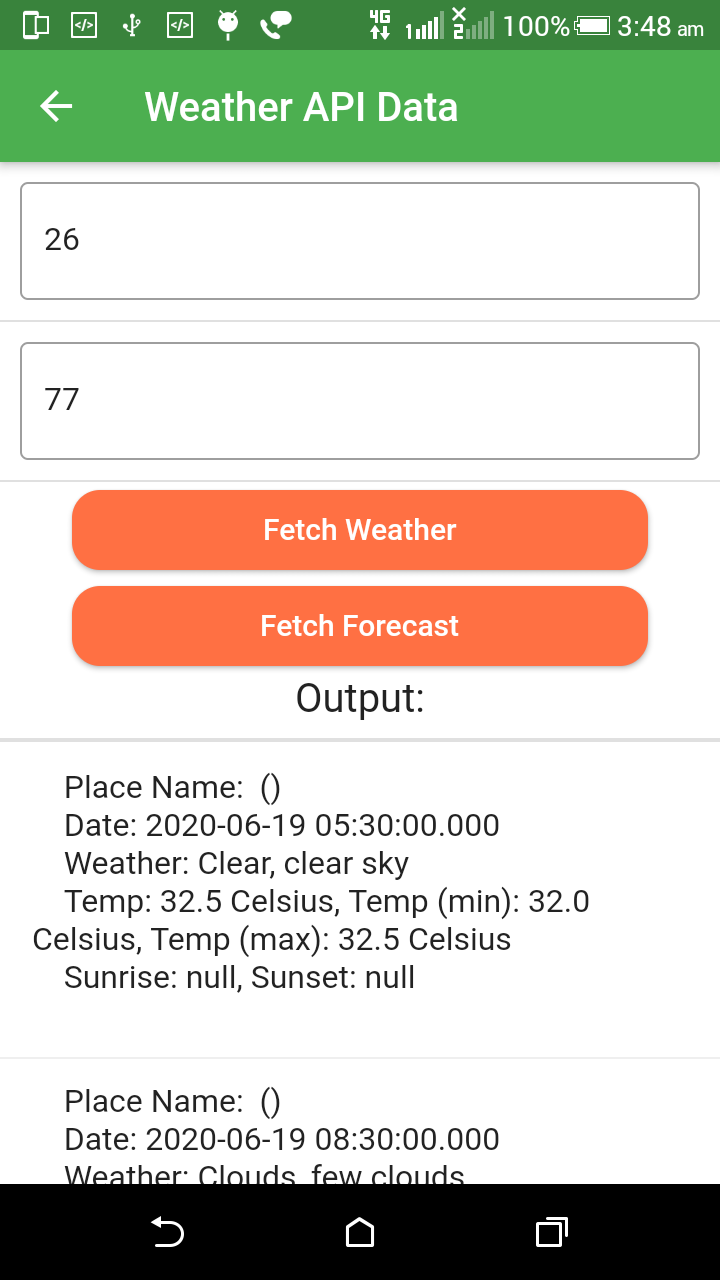
\includegraphics[height=10cm]{figures/weather-data.png}
\caption{\label{img417} Weather API data page}
\end{figure}

\subsection{Air Pollution Status}
When will be pressing on fourth RadioButton then will go to figure~\ref{img418} screenshot page basically this page is showing eight graphs that are temperature, humidity, air quality, carbon monoxide(CO), carbon dioxide($CO_{2}$),ammonium($NH_{4}$), smoke and LGP gas with respect to time.

\begin{figure}[!ht]
\centering
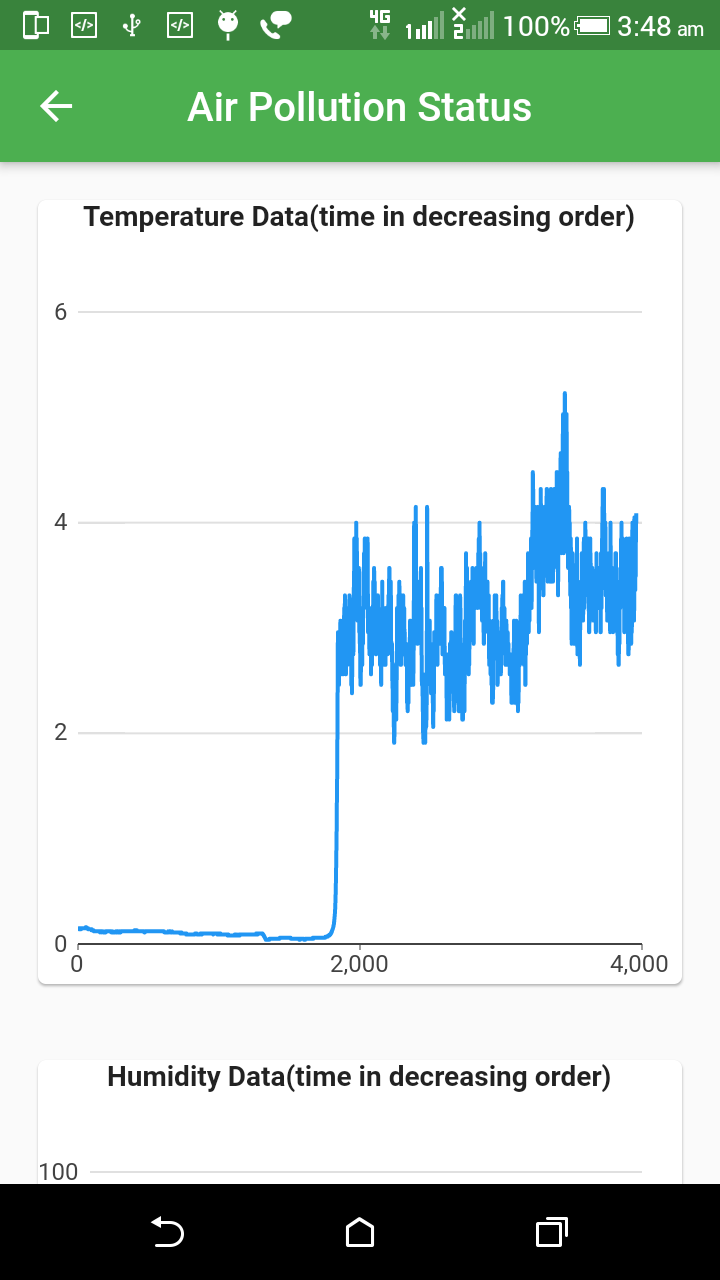
\includegraphics[height=10cm]{figures/pollution-status.png}
\caption{\label{img418} Weather API data page}
\end{figure}









% \label{chap4:intro}
% Research~\cite{wells+92} in science and technology has played a vital role in improvising human life at great extent. With the development of instrumentation and computation facilities, research on frontier areas has gone manifold. The discussion on the frontier areas of research in inter- disciplinary subject has always yielded novel ideas and collaborative research.


% \begin{figure}[!ht]
% \centering
% \includegraphics[scale=0.9]{car1.png}
% \caption{\label{img3} Image caption}
% \end{figure}

% Research in science and technology has played a vital role in improvising human life at great extent. With the development of instrumentation and computation facilities, research on frontier areas has gone manifold. The discussion on the frontier areas of research in inter- disciplinary subject has always yielded novel ideas and collaborative research. 

% \subsection{Test cases}
% Research in science and technology has played a vital role in improvising human life at great extent. With the development of instrumentation and computation facilities, research on frontier areas has gone manifold. The discussion on the frontier areas of research in inter- disciplinary subject has always yielded novel ideas and collaborative research.  








% %+++++++++++++++++++++++++++++++++++++++++++++++++++++++++++++++++++++++++++++++++
% \section{Summary}
% \label{chap4:sum}
% Research in science and technology has played a vital role in improvising human life at great extent. With the development of instrumentation and computation facilities, research on frontier areas has gone manifold. The discussion on the frontier areas of research in inter- disciplinary subject has always yielded novel ideas and collaborative research. In view of this, the First International Conference on Smart Technologies in Computer and Communication (SmartTech-2017) is meticulously planned to muster innovative ideas from researchers, scientists, academicians, Industry professionals and students. The aim of the conference is to provide a common platform to share and discuss the novel ideas, technologies and research findings to promote interdisciplinary research and to ignite young brains.


